\begin{wrapfigure}[0]{r}[9pt]{0cm}
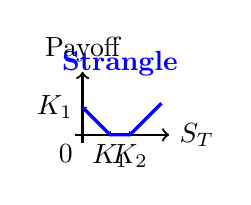
\begin{tikzpicture}[scale=1]
    % --- 定义坐标和参数 ---
    \def\Kone{0.35}       % 较低行权价 K1 (Put)
    \def\Ktwo{0.6}       % 较高行权价 K2 (Call), 确保 K1 < K2
    \def\maxST{1}      % S_T 的最大显示范围
    % 定义 Y 轴最大显示范围，稍微高过 K1 以便清楚显示截距
    \def\maxYAxis{0.8}

    % --- 绘制坐标轴 ---
    % Y 轴 (Payoff) - 收益始终 >= 0
    \draw[->, thick] (0, -0.1) -- (0, \maxYAxis) node[above] {Payoff};
    % X 轴 (S_T)
    \draw[->, thick] (-0.1, 0) -- (\maxST + 0.1, 0) node[right] {$S_T$};

    % --- 绘制辅助线和标签 ---
    % 标记原点
    \node[below left] at (0, 0) {0};

    % 在 X 轴上标记 K1
    \draw (\Kone, 0) node[below] {$K_1$} -- (\Kone, 0.05);

    % 在 X 轴上标记 K2
    \draw (\Ktwo, 0) node[below] {$K_2$} -- (\Ktwo, 0.05);

    % 在 Y 轴上标记 K1 (这是当 S_T=0 时，Put 的最大收益)
    \draw (0, \Kone) node[left] {$K_1$} -- (0.05, \Kone);

    % --- 绘制 Strangle 收益曲线 (蓝色粗线) ---
    % 路径分析:
    % 1. S_T < K1: 收益为 K1 - S_T。从 Y轴截距 (0, K1) 线性下降到 (K1, 0)。
    % 2. K1 <= S_T <= K2: 收益为 0。在 X 轴上从 (K1, 0) 平移到 (K2, 0)。
    % 3. S_T > K2: 收益为 S_T - K2。从 (K2, 0) 开始线性上升。
    %    为了视觉效果，终点选在 S_T = maxST 处，此时收益为 maxST - K2。
    \draw[blue, very thick] (0, \Kone) -- (\Kone, 0) -- (\Ktwo, 0) -- (\maxST, \maxST - \Ktwo);

    % --- 添加描述标签 (可选) ---
    % 左侧腿 (Put) 的描述


    % --- 添加标题标签 ---
    % 将标题放在图像上方居中位置 (在 K1 和 K2 中间上方)
    \node[blue, anchor=south, font=\bfseries,yshift=-5pt] at ({(\Kone+\Ktwo)/2}, \maxYAxis) {Strangle};

\end{tikzpicture}
\end{wrapfigure}